\chapter{Dyskusja rezultatów}

\section{Przykładowe wyniki}
\subsection{Wynik dla przykładu ze wstępu}
Wracając do dziennika zdarzeń przedstawionego w sekcji \ref{sec:event_logs}, a dla którego stworzono przykładowy model i obliczono metryki w sekcji \ref{sec:alignment-calculation}. 
\begin{figure}[!ht]
	\centering{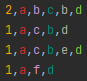
\includegraphics{datasets/v4a6c5l5.png}}
	\caption{\label{fig:flow_chart}Warianty procesu}
\end{figure}

Przy odkrywaniu modelu dla tego wariantu użyto następujących wag poszczególnych metryk: odwzorowanie = 18, złożoność = 2, generalizacja = 2, precyzja = 12, prostota = 2. Model dla tego dziennika zdarzeń znaleziony przy pomocy algorytmu to:
\begin{center}
	\{a\}xor(seq(opt(\{b\})\{c\}\{b\}opt(\{e\}))\{f\})\{d\}
\end{center}
oraz graficznie:

\begin{figure}[!ht]
	\centering{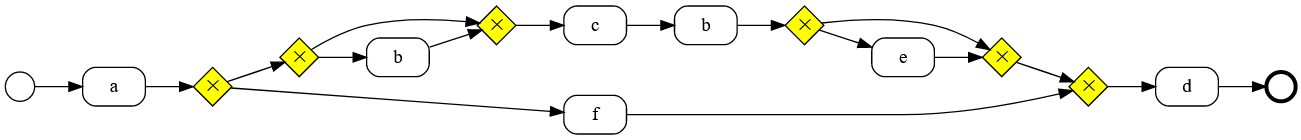
\includegraphics[scale=0.37]{examples/v4a6c5l5.csv_run-686_21_3_21_184242_35664_645567/graphviz.png}}
	\caption{\label{fig:flow_chart}Znaleziony model}
\end{figure}

Do znalezienia modelu potrzebne były 522 generacje, podczas których przeszukano 97771 unikalnych osobników. Zajęło to 1052.8 sekund, używając 4 wątków procesora. Natomiast, metryki mają następujące wartości: 

 \begin{center}
  \begin{tabular}{l}
	Średnia ważona: 0.9550 \\
	Odwzorowanie: 1.0 \\
	Złożoność: 1.0 \\
	Generalizacja: 0.3426 \\
	Precyzja: 0.9875 \\
	Prostota: 0.9231
  \end{tabular}
 \end{center}

Dla porównania poszczególne metryki obliczone w sekcji \ref{sec:alignment-calculation} wynosiły odwzorowanie = 0.9243, złożoność = 0.9706, generalizacja = 0.3997, precyzja = 0.9465, prostota = 0.8333, a średnia ważona używając przyjętych wag, wyniosłaby 0.9001. Otrzymano więc znacznie lepszy model.

Poniżej zaprezentowano również wykres, na który zaprezentowano zmianę wartości metryk w kolejnych generacjach. Jest on generowany podczas działania algorytmu i kończy się w momencie przerwania działania algorytmu, a znalezienia rozwiązania.
\begin{figure}[!ht]
	\centering{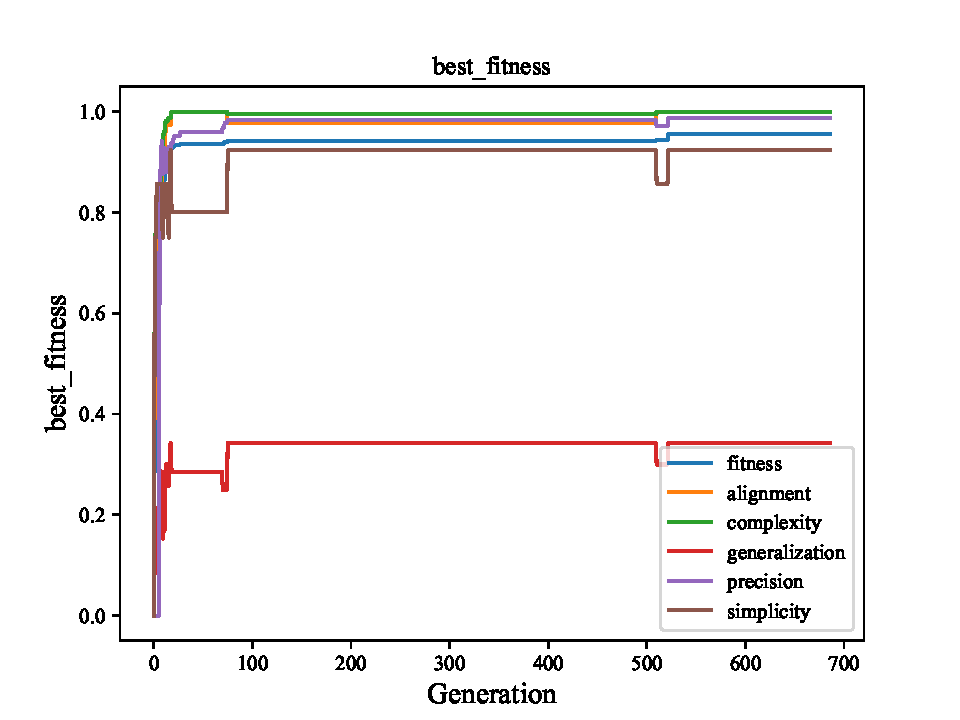
\includegraphics{examples/v4a6c5l5.csv_run-686_21_3_21_184242_35664_645567/best_fitness.pdf}}
	\caption{\label{fig:flow_chart}Przebieg ewolucji}
\end{figure}

\subsection{Inne przykłady działania}

Przykładowe dziennik zdarzeń wzięto z \cite{}. Część z nich została wygenerowania sztucznie, a część zawiera realne dane. Następnie log przerobiono na warianty procesu. 

\subsubsection{Przykład \#1}
\begin{figure}[!ht]
	\centering{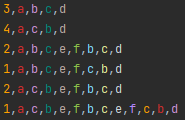
\includegraphics{datasets/v6a6c13l12.png}}
	\caption{\label{fig:flow_chart}Warianty procesu}
\end{figure}

Przy odkrywaniu modelu dla tego wariantu użyto następujących wag poszczególnych metryk: odwzorowanie = 18, złożoność = 2, generalizacja = 2, precyzja = 12, prostota = 2. Model dla tego dziennika zdarzeń znaleziony przy pomocy algorytmu to:
\begin{center}
	\{a\}xor(seq(opt(\{b\})\{c\}\{b\}opt(\{e\}))\{f\})\{d\}
\end{center}
oraz graficznie:

\begin{figure}[!ht]
	\centering{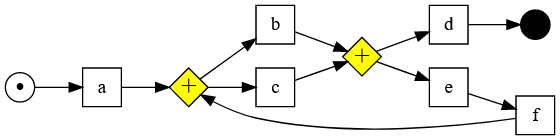
\includegraphics[scale=0.37]{examples/v6a6c13l12.csv_run-84_21_3_2_222502/graphviz.png}}
	\caption{\label{fig:flow_chart}Znaleziony model}
\end{figure}

Do znalezienia modelu potrzebne były 522 generacje, podczas których przeszukano 97771 unikalnych osobników. Zajęło to 1052.8 sekund, używając 4 wątków procesora. Natomiast, metryki mają następujące wartości: 

 \begin{center}
  \begin{tabular}{l}
	Średnia ważona: 0.9550 \\
	Odwzorowanie: 1.0 \\
	Złożoność: 1.0 \\
	Generalizacja: 0.3426 \\
	Precyzja: 0.9875 \\
	Prostota: 0.9231
  \end{tabular}
 \end{center}
 
\begin{figure}[!ht]
	\centering{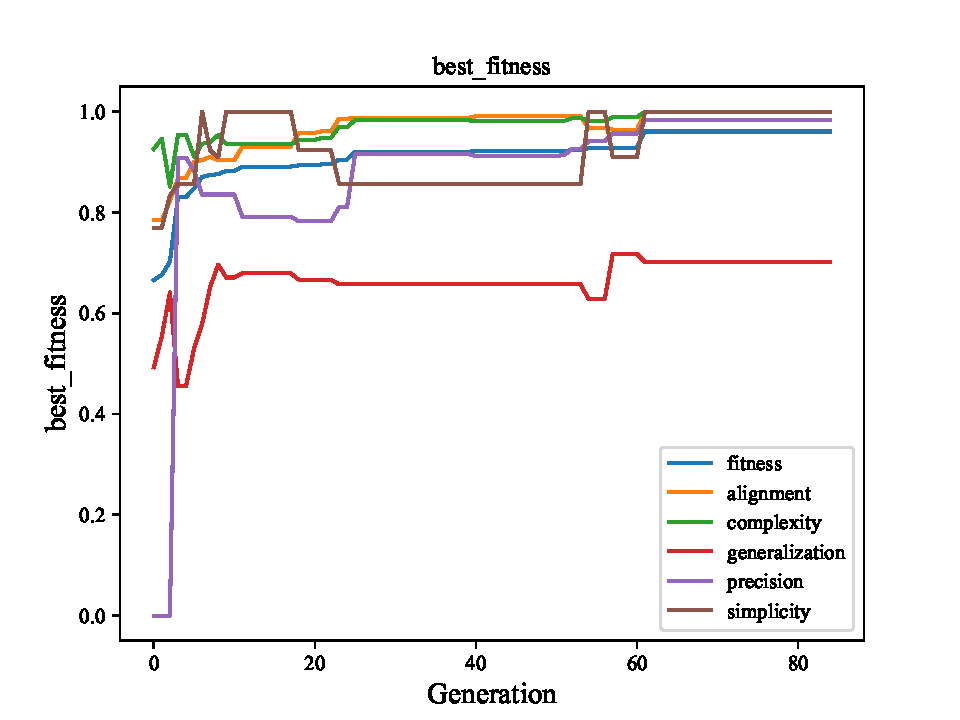
\includegraphics[scale=0.37]{examples/v6a6c13l12.csv_run-84_21_3_2_222502/best_fitness.pdf}}
	\caption{\label{fig:flow_chart}Przebieg ewolucji}
\end{figure}

\subsubsection{Przykład \#2}
\begin{figure}[!ht]
	\centering{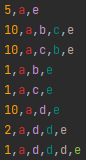
\includegraphics{datasets/v8a5c40l5.png}}
	\caption{\label{fig:flow_chart}Warianty procesu}
\end{figure}

Przy odkrywaniu modelu dla tego wariantu użyto następujących wag poszczególnych metryk: odwzorowanie = 18, złożoność = 2, generalizacja = 2, precyzja = 12, prostota = 2. Model dla tego dziennika zdarzeń znaleziony przy pomocy algorytmu to:
\begin{center}
	\{a\}xor(seq(opt(\{b\})\{c\}\{b\}opt(\{e\}))\{f\})\{d\}
\end{center}
oraz graficznie:

\begin{figure}[!ht]
	\centering{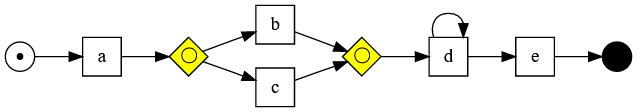
\includegraphics[scale=0.37]{examples/v8a5c40l5.csv_run-24_21_3_6_211037_47336_515221/graphviz.png}}
	\caption{\label{fig:flow_chart}Znaleziony model}
\end{figure}

Do znalezienia modelu potrzebne były 522 generacje, podczas których przeszukano 97771 unikalnych osobników. Zajęło to 1052.8 sekund, używając 4 wątków procesora. Natomiast, metryki mają następujące wartości: 

 \begin{center}
  \begin{tabular}{l}
	Średnia ważona: 0.9550 \\
	Odwzorowanie: 1.0 \\
	Złożoność: 1.0 \\
	Generalizacja: 0.3426 \\
	Precyzja: 0.9875 \\
	Prostota: 0.9231
  \end{tabular}
 \end{center}
 
\begin{figure}[!ht]
	\centering{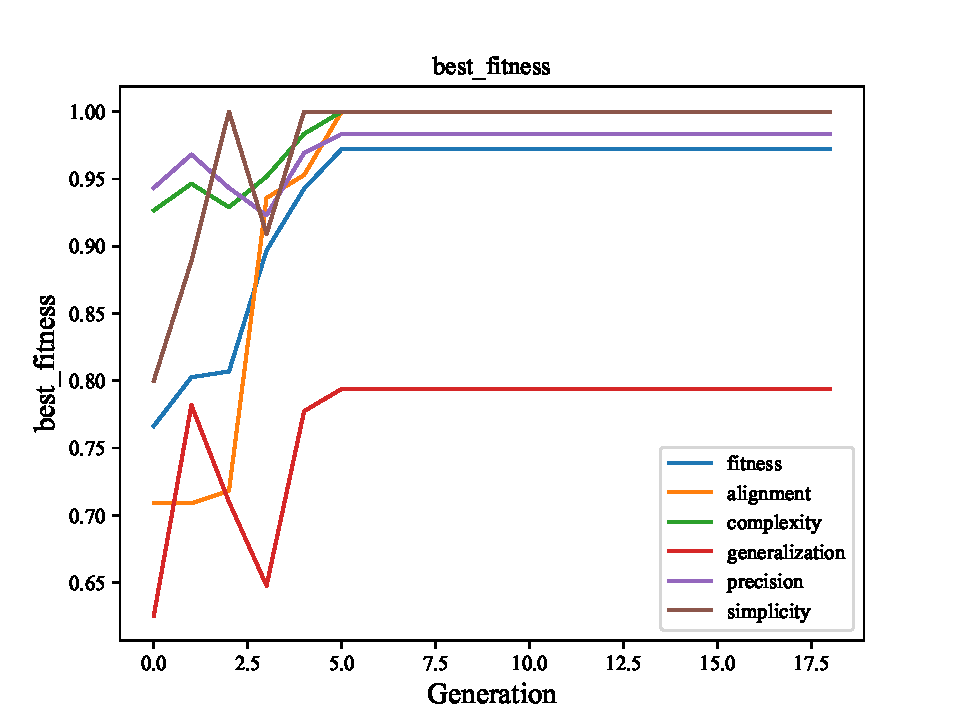
\includegraphics[scale=0.37]{examples/v8a5c40l5.csv_run-24_21_3_6_211037_47336_515221/best_fitness.pdf}}
	\caption{\label{fig:flow_chart}Przebieg ewolucji}
\end{figure}

\subsubsection{Przykład \#3}
\begin{figure}[!ht]
	\centering{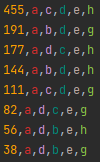
\includegraphics{datasets/v8a7c1254l5.png}}
	\caption{\label{fig:flow_chart}Warianty procesu}
\end{figure}

Przy odkrywaniu modelu dla tego wariantu użyto następujących wag poszczególnych metryk: odwzorowanie = 18, złożoność = 2, generalizacja = 2, precyzja = 12, prostota = 2. Model dla tego dziennika zdarzeń znaleziony przy pomocy algorytmu to:
\begin{center}
	\{a\}xor(seq(opt(\{b\})\{c\}\{b\}opt(\{e\}))\{f\})\{d\}
\end{center}
oraz graficznie:

\begin{figure}[!ht]
	\centering{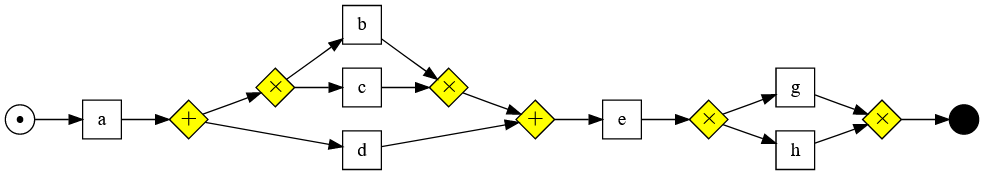
\includegraphics[scale=0.37]{examples/v8a7c1254l5.csv_run-303_21_3_5_003759/graphviz.png}}
	\caption{\label{fig:flow_chart}Znaleziony model}
\end{figure}

Do znalezienia modelu potrzebne były 522 generacje, podczas których przeszukano 97771 unikalnych osobników. Zajęło to 1052.8 sekund, używając 4 wątków procesora. Natomiast, metryki mają następujące wartości: 

 \begin{center}
  \begin{tabular}{l}
	Średnia ważona: 0.9550 \\
	Odwzorowanie: 1.0 \\
	Złożoność: 1.0 \\
	Generalizacja: 0.3426 \\
	Precyzja: 0.9875 \\
	Prostota: 0.9231
  \end{tabular}
 \end{center}
 
\begin{figure}[!ht]
	\centering{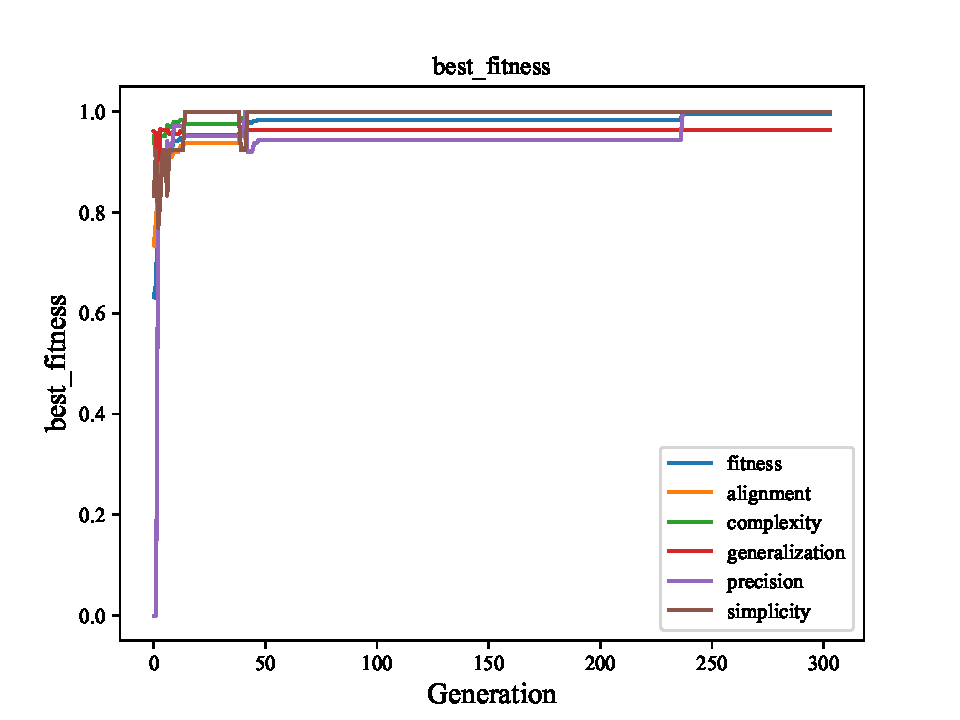
\includegraphics[scale=0.37]{examples/v8a7c1254l5.csv_run-303_21_3_5_003759/best_fitness.pdf}}
	\caption{\label{fig:flow_chart}Przebieg ewolucji}
\end{figure}

\subsubsection{Przykład \#4}
\begin{figure}[!ht]
	\centering{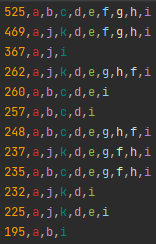
\includegraphics{datasets/v12a11c3512l9.png}}
	\caption{\label{fig:flow_chart}Warianty procesu}
\end{figure}

Przy odkrywaniu modelu dla tego wariantu użyto następujących wag poszczególnych metryk: odwzorowanie = 18, złożoność = 2, generalizacja = 2, precyzja = 12, prostota = 2. Model dla tego dziennika zdarzeń znaleziony przy pomocy algorytmu to:
\begin{center}
	\{a\}xor(seq(opt(\{b\})\{c\}\{b\}opt(\{e\}))\{f\})\{d\}
\end{center}
oraz graficznie:

\begin{figure}[!ht]
	\centering{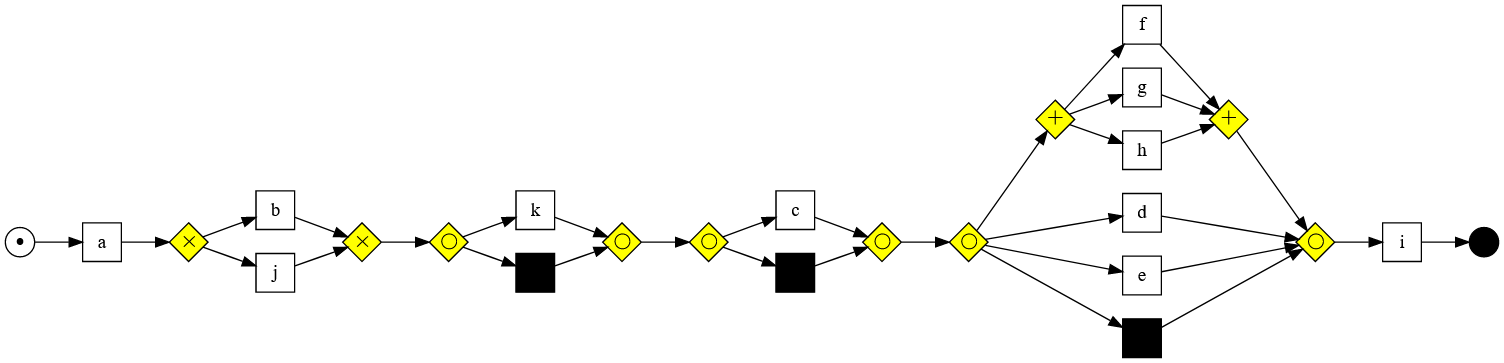
\includegraphics[scale=0.3]{examples/v12a11c3512l9.csv_run-10231_21_3_1_042344_29708_523416/graphviz.png}}
	\caption{\label{fig:flow_chart}Znaleziony model}
\end{figure}

Do znalezienia modelu potrzebne były 522 generacje, podczas których przeszukano 97771 unikalnych osobników. Zajęło to 1052.8 sekund, używając 4 wątków procesora. Natomiast, metryki mają następujące wartości: 

 \begin{center}
  \begin{tabular}{l}
	Średnia ważona: 0.9550 \\
	Odwzorowanie: 1.0 \\
	Złożoność: 1.0 \\
	Generalizacja: 0.3426 \\
	Precyzja: 0.9875 \\
	Prostota: 0.9231
  \end{tabular}
 \end{center}
 
\begin{figure}[!ht]
	\centering{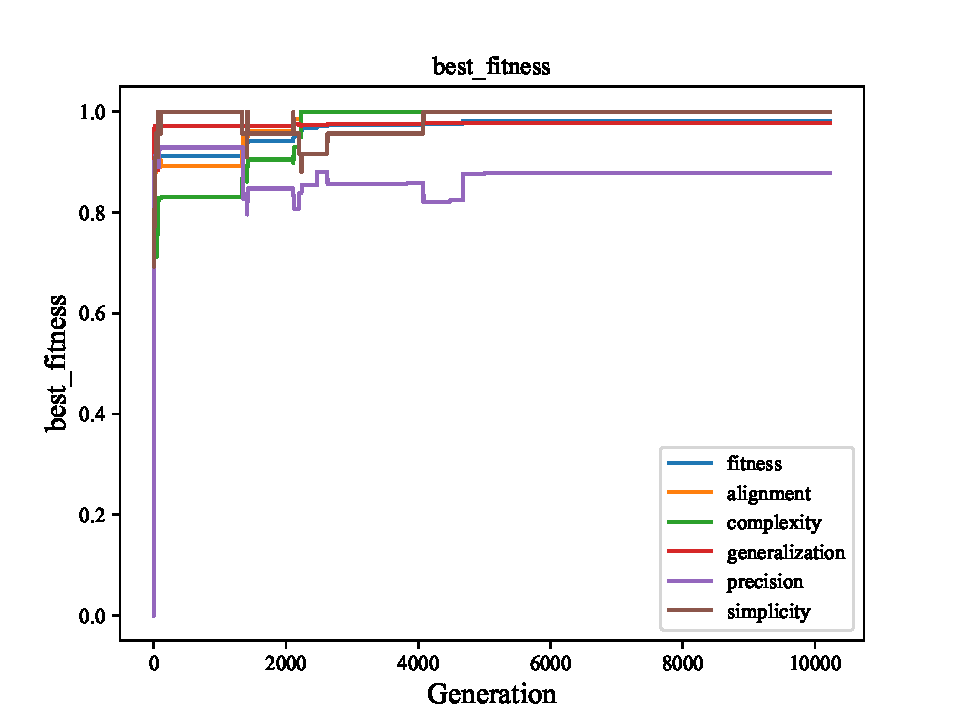
\includegraphics[scale=0.37]{examples/v12a11c3512l9.csv_run-10231_21_3_1_042344_29708_523416/best_fitness.pdf}}
	\caption{\label{fig:flow_chart}Przebieg ewolucji}
\end{figure}

\subsubsection{Przykład \#5}
\begin{figure}[!ht]
	\centering{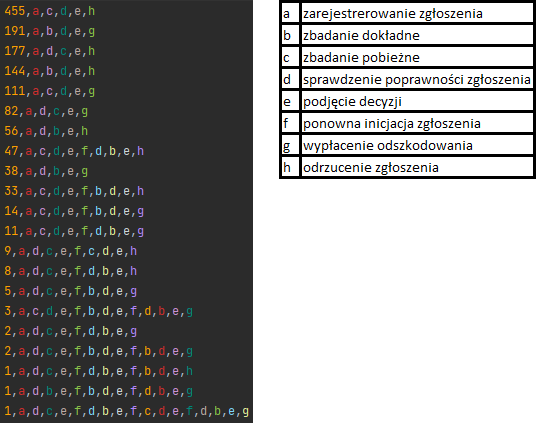
\includegraphics{datasets/v21a81391l17.png}}
	\caption{\label{fig:flow_chart}Warianty procesu}
\end{figure}

Przy odkrywaniu modelu dla tego wariantu użyto następujących wag poszczególnych metryk: odwzorowanie = 18, złożoność = 2, generalizacja = 2, precyzja = 12, prostota = 2. Model dla tego dziennika zdarzeń znaleziony przy pomocy algorytmu to:
\begin{center}
	\{a\}xor(seq(opt(\{b\})\{c\}\{b\}opt(\{e\}))\{f\})\{d\}
\end{center}
oraz graficznie:

\begin{figure}[!ht]
	\centering{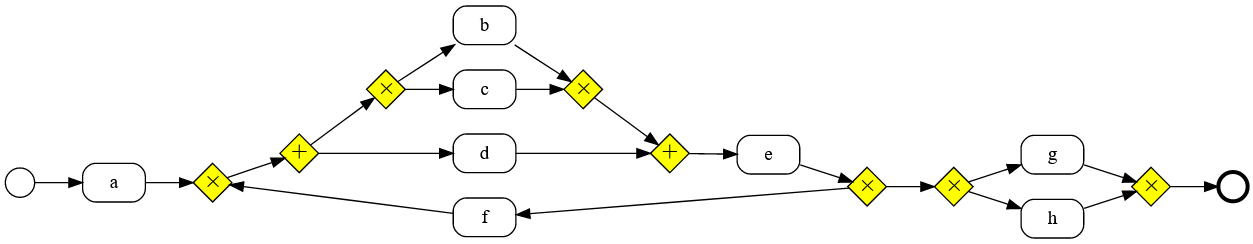
\includegraphics[scale=0.37]{examples/v21a81391l17.csv_run-15614_21_3_1_225455/graphviz.png}}
	\caption{\label{fig:flow_chart}Znaleziony model}
\end{figure}

Do znalezienia modelu potrzebne były 522 generacje, podczas których przeszukano 97771 unikalnych osobników. Zajęło to 1052.8 sekund, używając 4 wątków procesora. Natomiast, metryki mają następujące wartości: 

 \begin{center}
  \begin{tabular}{l}
	Średnia ważona: 0.9550 \\
	Odwzorowanie: 1.0 \\
	Złożoność: 1.0 \\
	Generalizacja: 0.3426 \\
	Precyzja: 0.9875 \\
	Prostota: 0.9231
  \end{tabular}
 \end{center}
 
\begin{figure}[!ht]
	\centering{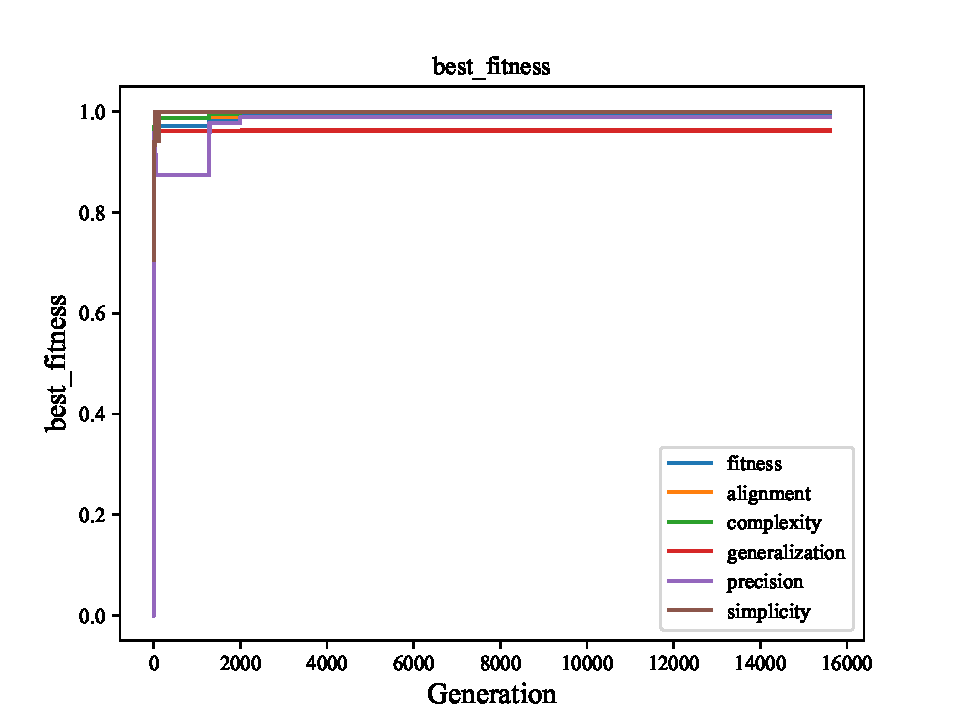
\includegraphics[scale=0.37]{examples/v21a81391l17.csv_run-15614_21_3_1_225455/best_fitness.pdf}}
	\caption{\label{fig:flow_chart}Przebieg ewolucji}
\end{figure}

\subsubsection{Przykład \#6}
\begin{figure}[!ht]
	\centering{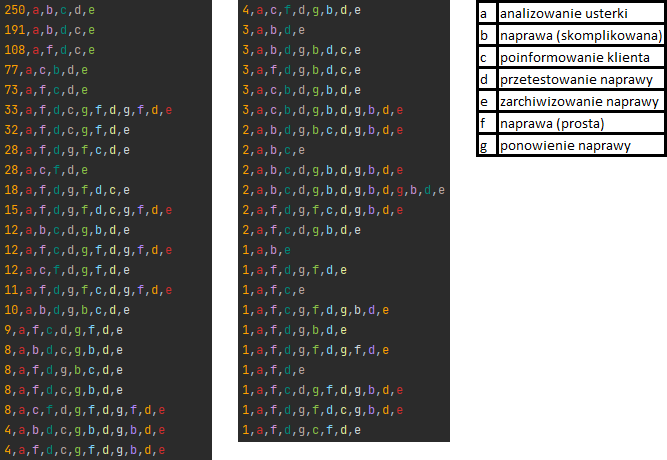
\includegraphics{datasets/v45a7c1000l14.png}}
	\caption{\label{fig:flow_chart}Warianty procesu}
\end{figure}

Przy odkrywaniu modelu dla tego wariantu użyto następujących wag poszczególnych metryk: odwzorowanie = 18, złożoność = 2, generalizacja = 2, precyzja = 12, prostota = 2. Model dla tego dziennika zdarzeń znaleziony przy pomocy algorytmu to:
\begin{center}
	\{a\}xor(seq(opt(\{b\})\{c\}\{b\}opt(\{e\}))\{f\})\{d\}
\end{center}
oraz graficznie:

\begin{figure}[!ht]
	\centering{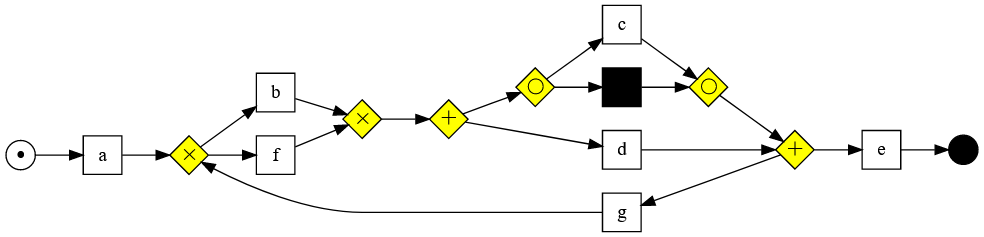
\includegraphics[scale=0.37]{examples/v45a7c1000l14.csv_run-1366_21_3_6_143708_2144_563150/graphviz.png}}
	\caption{\label{fig:flow_chart}Znaleziony model}
\end{figure}

Do znalezienia modelu potrzebne były 522 generacje, podczas których przeszukano 97771 unikalnych osobników. Zajęło to 1052.8 sekund, używając 4 wątków procesora. Natomiast, metryki mają następujące wartości: 

 \begin{center}
  \begin{tabular}{l}
	Średnia ważona: 0.9550 \\
	Odwzorowanie: 1.0 \\
	Złożoność: 1.0 \\
	Generalizacja: 0.3426 \\
	Precyzja: 0.9875 \\
	Prostota: 0.9231
  \end{tabular}
 \end{center}
 
\begin{figure}[!ht]
	\centering{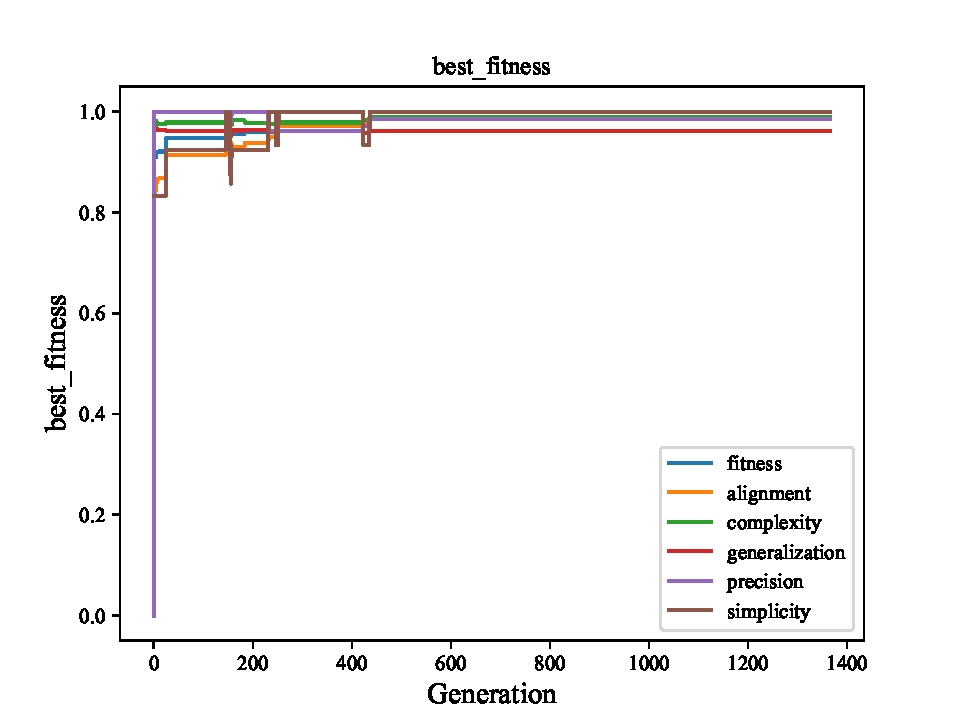
\includegraphics[scale=0.8]{examples/v45a7c1000l14.csv_run-1366_21_3_6_143708_2144_563150/best_fitness.pdf}}
	\caption{\label{fig:flow_chart}Przebieg ewolucji}
\end{figure}


\section{Wyniki w zależności od przyjętych wag poszczególnych metryk}

\subsection{Złożoność}

\section{Wnioski}
